% kuleuventheme2 by Janez Kren, September 2017, janez.kren@kuleuven.be, based on:
% kuleuventheme 1.3 by Roland Pastorino, 2013 roland.pastorino@kuleuven.be / www.rolandpastorino.com

%\documentclass[10pt,t]{beamer} %print pause
\documentclass[handout,10pt,t]{beamer}  %unprint pause
\usetheme{kuleuven2}	%THEME OPTIONS for LOGO: kul (default), kulak, lrd,    ; OPTIONS for TITLE PAGE: normal (default), sedes


%%% OTHER SETTINGS
\usefonttheme[onlymath]{serif}			% math font with serifs, delete to make it sans-serif
\setbeamertemplate{footline}[body] 		% delete this line to remove footline bar on all frames
%\usepackage[orientation=landscape,size=custom,width=16,height=9,scale=0.5,debug]{beamerposter} %enable for widescreen 16:9 ratio
\titlegraphic{ 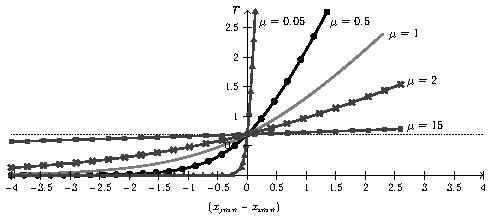
\includegraphics[width=0.001\paperwidth]{TikZFigures/scale_param_effect.pdf} } %optional title page image

%%% ADDED PACKAGES:
\usepackage[english]{babel}
\usepackage{amsfonts}
\usepackage{amssymb}


%%% Added alvaro
\usepackage{fancyvrb} %inline verbatim...



%multi-row
\usepackage{multirow}
\usepackage{bigstrut}


\usepackage{fontawesome} %icons, twitter, etc...
\usepackage{stata} % StataStyle (need to be placed on the folde)
%Colors
\usepackage{hyperref}
\hypersetup{
	colorlinks=true,
	linkcolor=blue,
	filecolor=blue,
	citecolor = blue,      
	urlcolor=cyan,
}
%color for ticket
\definecolor{applegreen}{rgb}{0.55, 0.71, 0.0}

%references style
\usepackage{natbib}
\bibliographystyle{apalike}
% make bibliography entries smaller
\renewcommand\bibfont{\scriptsize}
% If you have more than one page of references, you want to tell beamer
% to put the continuation section label from the second slide onwards
\setbeamertemplate{frametitle continuation}[from second]
% Now get rid of all the colours
\setbeamercolor*{bibliography entry title}{fg=black}
\setbeamercolor*{bibliography entry author}{fg=black}
\setbeamercolor*{bibliography entry location}{fg=black}
\setbeamercolor*{bibliography entry note}{fg=black}
% and kill the abominable icon
\setbeamertemplate{bibliography item}{}

%% square images
\usepackage{tikz}
\usetikzlibrary{tikzmark,decorations.pathmorphing}


%% Snippet for \pause on align enviroment 
\makeatletter
\let\save@measuring@true\measuring@true
\def\measuring@true{%
	\save@measuring@true
	\def\beamer@sortzero##1{\beamer@ifnextcharospec{\beamer@sortzeroread{##1}}{}}%
	\def\beamer@sortzeroread##1<##2>{}%
	\def\beamer@finalnospec{}%
}
\makeatother

%% Creating checkmark
\def\checkmark{\tikz\fill[scale=0.4](0,.35) -- (.25,0) -- (1,.7) -- (.25,.15) -- cycle;} 

%% Creating highlight text 
\usepackage{soul}
\makeatletter
\let\HL\hl
\renewcommand\hl{%
	\let\set@color\beamerorig@set@color
	\let\reset@color\beamerorig@reset@color
	\HL}
\makeatother
%%highlight with pause
\renewcommand<>{\hl}[1]{\only#2{\beameroriginal{\hl}}{#1}}



%% Creating danger mark 
\newcommand*{\TakeFourierOrnament}[1]{{%
		\fontencoding{U}\fontfamily{futs}\selectfont\char#1}}
\newcommand*{\danger}{\TakeFourierOrnament{66}}


%%
\usepackage{ragged2e}
\usepackage{etoolbox}
\apptocmd{\frame}{}{\justifying}{} % Allow optional arguments after frame.




%%% TITLE PAGE INFO:
\title[Zhu, Guti\'errez-Vargas \& Vandebroek: Mixed random regret minimization models.]{Fitting mixed random regret minimization models using \texttt{mixrandregret}. } %[]] will appear in footline
\subtitle{UK Stata Meeting - London, 2022. \\ \small{Presenter: Álvaro A. Gutiérrez-Vargas } }
\author{$\bullet$ Ziyue Zhu {\color{black}(\href{https://github.com/ziyue16}{ \faGithub},  \href{https://www.linkedin.com/in/ziyue-zhu-397a67109/}{\faLinkedinSquare })'} \\ 
	$\bullet$ \'Alvaro A. Guti\'errez-Vargas {\color{black}(\href{https://github.com/alvarogutyerrez}{ \faGithub},  \href{https://www.linkedin.com/in/alvarogutierrezvargas/}{\faLinkedinSquare })'} \\ $\bullet$ Martina Vandebroek }	
\institute{\faMapMarker   \scriptsize{ Research Centre for Operations Research and Statistics (\href{https://feb.kuleuven.be/research/decision-sciences-and-information-management/orstat/orstat}{ORSTAT})}}
\date{}




\begin{document}
\csname beamer@calculateheadfoot\endcsname %recalculate head and foot dimension


 %%
 %%  0. TITLE PAGE and TABLE OF CONTENT
 %%
% Title page

\begin{frame}[plain,noframenumbering]
	\titlepage
\end{frame}
	


% Table of Contents

\begin{frame}[noframenumbering]{}
	\hfill	{\small \parbox{.961\textwidth}{\tableofcontents[hideothersubsections]}}
\end{frame}


\section{Random Regret Minimization Models}



\begin{frame}{ \textit{What is Regret and how to use it for Choice Modeling?} }
	
	\begin{itemize}
	\item From Utility to Regret.\pause
	\item Regret: Situation where a \hl{non-chosen alternative ends up being more attractive than the chosen one}\pause
	\item Individuals are assumed to minimize regret.\pause		
	\end{itemize}
	

	\begin{table}[h!] 
		\centering
		\caption{\small{Hypothetical Choice Situation}\label{tab_choice_task_1_ex}}
		\scalebox{0.75}{\begin{tabular}{|c|c|c|c|}\hline
				Attribute $\backslash$  Route & 1 &2 &3  \\ \hline \hline
				Travel Time  & 23 min. & 27 min. & 35 min. \\ \hline
				Travel Cost  & 6 euros  &4 euros &3 euros \\  \hline 
		\end{tabular}}
	\end{table}
	If we chose alternative $2$:
	\begin{itemize}
		\pause \item Alternative $1$ is faster...
		\pause \item Alternative $3$ is cheaper...
	\end{itemize}
	\pause \hl{ $\Rightarrow$ RRM models will (formalize and) minimize this notion of regret!}
\end{frame}



\begin{frame}{Formalization of the later example.}
	\begin{table}[h!] 
		\centering
		\scalebox{0.85}{\begin{tabular}{|c|c|c|c|}\hline
				Attribute $\backslash$  Route & 1 &2 &3  \\ \hline \hline
				Travel Time  & 23 min. & 27 min. & 35 min. \\ \hline
				Travel Cost  & 6 euros  &4 euros &3 euros \\  \hline 
		\end{tabular}}
		\caption{Hypothetical Choice Situation\label{tab_choice_task_1_ex}}
	\end{table}
	We will denote in the following:
	
	
	\begin{itemize}
		\item Decision-makers (referred to $n$) answer $s$ choice situations \pause \medskip
		\item They decide among $J$ alternatives (referred to $i$ or $j$ indistinctly).\pause\medskip
		\item Each alternative is described by $M$ attributes (referred to $m$).\pause\medskip
		\item \hl{$x_{ins,m}$} The value of attribute $m$ of alternative $i$ for individual $n$ in choice situation $s$ is denoted by .\pause
	\end{itemize}

	\begin{itemize}
		\item \hl{$y_{ins}$} is the response variable that takes the value of 1 when alternative $i$ is chosen by individual $n$ in choice situation $s$ and 0 otherwise.
	\end{itemize}
\end{frame}








\subsection{Random Utility  vs Random Regret }


\begin{frame}{RUM vs RRM}
	\begin{itemize}
		\item Random Utility Maximization (RUM)
		\pause
		\begin{align*}
		\tikzmarknode{utilityfn}{U_{ins}} &= \tikzmarknode{systematutilityfn}{V_{ins}} + \varepsilon_{ins}  \pause \\
		&=
		\beta_{n,\boldsymbol{T}}\times x_{ins,\boldsymbol{T}} 
		+ 
		\beta_{n,\boldsymbol{C}}\times x_{ins,\boldsymbol{C}} 
		+ 
		\varepsilon_{ins}
		\end{align*}
		\pause
		\begin{tikzpicture}[overlay,remember picture,decoration={segment
			length=1pt,amplitude=0.4pt},red]
		\draw[decorate,->] (systematutilityfn)
		to[out=40,in=-180] ++ (1.5,0.55) node[right,<->]{Systematic Utility};
		\end{tikzpicture}
		\pause
		\begin{tikzpicture}[overlay,remember picture,decoration={segment
			length=1pt,amplitude=0.4pt},red]
		\draw[decorate,->] (utilityfn)
		to[out=-100,in=0] ++ (-1.5,0) node[left,<->]{Utility};
		\end{tikzpicture}
		\pause
		\item Random Regret Minimization (RRM)
		\pause
		\begin{align*}
		\tikzmarknode{regretfn}{RR_{ins}} &= \tikzmarknode{systematregretfn}{R_{ins}} + \varepsilon_{ins}\\
		&=
		\sum_{j\neq i }^{J}R_{i\leftrightarrow j n s,  \boldsymbol{T}} 
		+ 
		\sum_{j\neq i }^{J}R_{i\leftrightarrow j n s, \boldsymbol{T}} 
		+ 
		\varepsilon_{ins}
		\end{align*}
		\pause
		\begin{tikzpicture}[overlay,remember picture,decoration={segment
			length=1pt,amplitude=0.4pt},red]
		\draw[decorate,->] (systematregretfn)
		to[out=40,in=180] ++  (1.5,0.55)  node[right,<-]{Systematic Regret};
		\end{tikzpicture}
		\pause
		\begin{tikzpicture}[overlay,remember picture,decoration={segment
			length=1pt,amplitude=0.4pt},red]
		\draw[decorate,->] (regretfn)
		to[out=-100,in=0] ++ (-1.5,0) node[left,<->]{Regret};
		\end{tikzpicture}
		\pause
		\begin{itemize}
			\item 	The \hl{notion of \textit{regret}} is characterize by the systematic regret $R_{ins}$. \pause
			\medskip
			\item $R_{in}$ is described in terms of \textit{\textbf{attribute level regret}} ($R_{i\leftrightarrow j ns,m}$).\pause\medskip
		\end{itemize}
	\end{itemize}
\end{frame}



%\subsection{Early RRM Model }
%\begin{frame}{Early Model 	\citep{Chorus_2008}}
%	{\color{cyan}{$\bullet$}} \citep{Chorus_2008} proposed the following systematic regret:
%	\begin{align}\label{eq:RRM_max}
%	R^{\max}_{in} &= 
%	\max_{j\neq i}\left\{ \sum_{m=1}^{M} 	\tikzmarknode{attriblevelmax}{R^{\max}_{i\leftrightarrow j,mn}} \right\}
%	=
%	\max_{j\neq i}\left\{   \sum_{m=1}^{M} \max\left\{0,\tikzmarknode{coefficientmax}{\beta_{m}}\cdot\left(x_{jmn} - x_{imn}\right)\right\} \right\} 
%	\end{align}\pause
%	
%	\begin{tikzpicture}[overlay,remember picture,decoration={segment
%		length=1pt,amplitude=0.4pt},red]
%	\draw[decorate,->] (coefficientmax)
%	to[out=-40,in=0] ++ (0.55,-0.75) node[left,<->]{Regret Coefficient attribute $m$};
%	\end{tikzpicture}\pause
%	\begin{tikzpicture}[overlay,remember picture,decoration={segment
%		length=1pt,amplitude=0.4pt},red]
%	\draw[decorate,->] (attriblevelmax)
%	to[out=-40,in=0] ++  (-0.75,-0.75)  node[left,->]{Attribute level regret };
%	\end{tikzpicture}\pause
%	%\begin{itemize}
%	%	\item Being $\mathcal{M} = \left\{t,c\right\}$(Attributes), $\mathcal{J} = \left\{1,2,3\right\}$(Alternatives). 
%	%	\item The regret of alternative 1 ($R^{\max}_{1}$) will be described by the following:
%	%\end{itemize}
%	Assumptions being made here:\\
%	
%	{\color{cyan}{$\bullet$}} The regret is only produced by the best non-chosen alternative (outer $\max$).\pause 
%	
%	{\color{cyan}{$\bullet$}} Regret increases linear with the differences in the pairwise comparison of alternatives (inner $\max$).\\ \pause
%	
%		Possible difficulties/problems: \\
%		
%{\color{cyan}{$\bullet$}} The max operator is not differentiable $\Rightarrow$ non-smooth log-likelihood\pause 
%
%{\color{cyan}{$\bullet$}} Why just the best non-chose alternative? What about all the others?\pause 
%
%\end{frame}
%
%
%
%
%\subsection{Early RRM Model }
%\begin{frame}{Early Model 	\citep{Chorus_2008}: An example.}
%	{\color{cyan}{$\bullet$}} \citep{Chorus_2008} proposed the following systematic regret:
%	\begin{align}\label{eq:RRM_max}
%	R^{\max}_{in} &= 
%	\max_{j\neq i}\left\{ \sum_{m=1}^{M} 	\tikzmarknode{attriblevelmax}{R^{\max}_{i\leftrightarrow j,mn}} \right\}
%	=
%	\max_{j\neq i}\left\{   \sum_{m=1}^{M} \max\left\{0,\tikzmarknode{coefficientmax}{\beta_{m}}\cdot\left(x_{jmn} - x_{imn}\right)\right\} \right\} 
%	\end{align}\pause
%		
%	\begin{tikzpicture}[overlay,remember picture,decoration={segment
%		length=1pt,amplitude=0.4pt},red]
%	\draw[decorate,->] (coefficientmax)
%	to[out=-40,in=0] ++ (0.55,-0.75) node[left,<->]{Regret Coefficient attribute $m$};
%	\end{tikzpicture}
%	\begin{tikzpicture}[overlay,remember picture,decoration={segment
%		length=1pt,amplitude=0.4pt},red]
%	\draw[decorate,->] (attriblevelmax)
%	to[out=-40,in=0] ++  (-0.75,-0.75)  node[left,->]{Attribute level regret };
%	\end{tikzpicture}\pause
%%\begin{itemize}
%%	\item Being $\mathcal{M} = \left\{t,c\right\}$(Attributes), $\mathcal{J} = \left\{1,2,3\right\}$(Alternatives). 
%%	\item The regret of alternative 1 ($R^{\max}_{1}$) will be described by the following:
%%\end{itemize}
%	
%{\color{cyan}{$\bullet$}} From our example $\mathcal{M} = \left\{t,c\right\}$(Attributes), $\mathcal{J} = \left\{1,2,3\right\}$(Alternatives).\pause 	\\
%{\color{cyan}{$\bullet$}} For instance: Regret of alternative 1  ($R^{\max}_{1}$) will be described by:\pause
%
%\scalebox{1}{\parbox{1\linewidth}{%
%\begin{align*}
%R^{\max}_{1} & = 
%\max\left\{
%\left({\color{blue}{\sum_{m\in\mathcal{M}} 	R^{\max}_{1\leftrightarrow 2,m}}} \right),
%\left({\color{red}{\sum_{m\in\mathcal{M}} 	R^{\max}_{1\leftrightarrow 3,m}}} \right)
%\right\}\\ 
%&=\max\left\{
%\color{blue}{ \left(R^{\max}_{1\leftrightarrow 2, t}+R^{\max}_{1\leftrightarrow 2, c}\right)}
%\boldsymbol{,}
%\color{red}{\left(R^{\max}_{1\leftrightarrow 3, t}+R^{\max}_{1\leftrightarrow 3, c}\right)}\right\}  \\ 
%& = \max\left\{\right.
%\color{blue}{\left(\max\left\{ 0,\beta_{t}\left(x_{2,t}-x_{1,t}\right) \right\} +  \max\left\{ 0,\beta_{c}\left(x_{2,c}-x_{1,c}\right) \right\}\right)}, \\ 
%&\;\;\;\;\;\;\;\;\;\;\;\;\;\;\left(\color{red}{\max\left\{ 0,\beta_{t}\left(x_{3,t}-x_{1,t}\right) \right\} +  \max\left\{ 0,\beta_{c}\left(x_{3,c}-x_{1,c}\right) \right\}}\right)
%\left.\right\}
%\end{align*}}}
%\end{frame}
%
%
%
%
%\begin{frame}{Early Model 	\citep{Chorus_2008}: Log-likelihood.}
%\begin{itemize}
%\item  Defining $RR^{\max}_{in} =R^{\max}_{in} + \varepsilon_{in}$, where $\varepsilon_{in}$ is a type I Extreme Value i.i.d. error.\pause
%\item Acknowledging that the minimization of the random regret is mathematically equivalent to maximizing the negative of the regret.\pause
%\item Hence, the probabilities may be derived using the Multinomial Logit:	
%\end{itemize}
%
%
%\scalebox{0.85}{\parbox{1\linewidth}{%
%\begin{align}\label{eq:RRM_max_pbb}
%P^{\max}_{in} = \dfrac{\exp{\left(-R^{\max}_{in}\right)}}{\sum_{j=1}^{J} \exp{\left(-R^{\max}_{jn}\right)}} & &\text{for }i=1,\dots,J
%\end{align}}}
%
%\pause
%\begin{itemize}
%\item Consequently, the log-likelihood will be described by:
%\end{itemize}
%
%\scalebox{0.85}{\parbox{1\linewidth}{%
%\begin{align*}\label{eq:loglikelihood}
%\ln L &= \sum_{n=1}^{N}\sum_{i=1}^{J}
%y_{in}\ln
%\left(
%P^{\max}_{in}
%\right)
%\nonumber\\	
%&
%=-\sum_{n=1}^{N} \sum_{i=1}^{J} y_{in}  R^{\max}_{in}
%-\sum_{n=1}^{N}\sum_{i=1}^{J} y_{in}
%\ln
%\left(
%\sum_{j=1}^{J}\exp\left(- R^{\max}_{jn}\right)
%\right)
%\end{align*}}}
%\end{frame}




\begin{frame}{\textbf{\textit{The Attribute level regret}}  $R_{i\leftrightarrow j ns,m}$}
	\begin{table}[h!] 
	\centering
	\scalebox{0.75}{\begin{tabular}{|c|c|c|c|}\hline
			Attribute $\backslash$  Route & 1 &2 &3  \\ \hline \hline
			Travel Time  & 23 min. & 27 min. & 35 min. \\ \hline
			Travel Cost  & 6 euros  &4 euros &3 euros \\  \hline 
	\end{tabular}}
\begin{itemize}
	\item $R_{i\leftrightarrow j , mn}$ describes the \hl{pairwise combinations of regret derived from alternatives}.
\end{itemize}

\end{table}
\pause
\begin{table}[h!]
	\centering
	\scalebox{0.758}{\begin{tabular}{|c|c|c|c|c|}
		\hline
		\multicolumn{1}{|c|}{	\textbf{$(x_{jns,m}-x_{{\color{red}{{\boldsymbol{i}}}}ns,m})$}} & Attribute \textbackslash{} Route & $j=1$     & $j=2$     & $j=3$ \bigstrut\\
		\hline
		\hline
		$(x_{jns,m}-x_{{\color{red}{{\boldsymbol{1}}}}ns,T})$     & Travel Time & \textcolor[rgb]{ 1,  0,  0}{0} & 4     & 12 \bigstrut\\
		\hline
		$(x_{jns,m}-x_{{\color{red}{{\boldsymbol{1}}}}ns,C})$    & Travel Cost & \textcolor[rgb]{ 1,  0,  0}{0} & -2    & -3 \bigstrut\\
		\hline\hline
		$(x_{jns,m}-x_{{\color{red}{{\boldsymbol{2}}}}ns,T})$     & Travel Time & -4    & \textcolor[rgb]{ 1,  0,  0}{0} & 8 \bigstrut\\
		\hline
		$(x_{jns,m}-x_{{\color{red}{{\boldsymbol{2}}}}ns,C})$& Travel Cost & 2     & \textcolor[rgb]{ 1,  0,  0}{0} & -1 \bigstrut\\
		\hline\hline
		$(x_{jns,m}-x_{{\color{red}{{\boldsymbol{3}}}}ns,T})$     & Travel Time & -12   & -8    & \textcolor[rgb]{ 1,  0,  0}{0} \bigstrut\\
		\hline
		$(x_{jns,m}-x_{{\color{red}{{\boldsymbol{3}}}}ns,C})$& Travel Cost & 3     & 1     & \textcolor[rgb]{ 1,  0,  0}{0} \bigstrut\\
		\hline
	\end{tabular}}
	\label{tab:addlabel}%
\end{table}%
\pause
\begin{itemize}
	\item \hl{Takeaway}: We will define $R_{i\leftrightarrow j ns,m}$ in terms of the attribute differences.
\end{itemize}
\end{frame}


\begin{frame}{Classical RRM 	\citep{chorus2010}}

\begin{itemize}
	\item 	\citep{chorus2010} proposed the following attribute level regret: 
$$R_{i\leftrightarrow j ns,m} =	\ln
\left[
1 + \exp
\left\{
\beta_{n,m}\cdot\left(x_{jns,m} - x_{ins,m}\right)
\right\}
\right] $$
	\item 	$R_{i\leftrightarrow j ns,m}$ compares alternative $i$ with alternative $j$ in attribute $m$.\pause
	\medskip
	\item $\sum_{j\neq i }R_{i\leftrightarrow jns,m}$ is the equivalent to $x_{ins,m}\times\beta_{n,m}$ in an utilitarian model. \pause
	\medskip	
\item $\beta_{n,m}$ is the taste parameter of attribute $m$ of individual $n$. 
\end{itemize}

\end{frame}



%\begin{frame}{ Classical RRM 	\citep{chorus2010}.}
%	\begin{figure}
%		\centering
%		\includegraphics[width=0.9\linewidth]{../../randregret_submission/article/tikz_figures/non_compensatory_effect}
%		\caption{ $R_{i \leftrightarrow j, mn}$ conditional on $\beta_{m}=1$.}
%	\end{figure}
%\end{frame}





\subsection{Classical Regret Function}
\begin{frame}{Classical RRM 	\citep{chorus2010}}
	
	{\color{cyan}{$\bullet$}}  \citep{chorus2010}	proposed the following systematic regret:    
	
	\begin{align}\label{eq:RRM_classic}
	R_{ins} &= 
	\sum_{j\neq i }^{J}   \tikzmarknode{sumclassicRRM}{\sum_{m=1}^{M}}\tikzmarknode{atributlevelclassicRRM}{R_{i\leftrightarrow j ns,m}}
	=
	\sum_{j\neq i }^{J}   \sum_{m=1}^{M}
	\ln
	\left[
	1 + \exp
	\left\{
	\beta_{n,m}\cdot\left(x_{jns,m} - x_{ins,m}\right)
	\right\}
	\right]
	\end{align}
	\pause
		\begin{tikzpicture}[overlay,remember picture,decoration={segment
		length=1pt,amplitude=0.4pt},red]
	\draw[decorate,->] (atributlevelclassicRRM)
	to[out=150,in=-500] ++  (0.15,0.95)  node[right,->]{Attribute level regret. };
	\end{tikzpicture}
	\pause
	\begin{tikzpicture}[overlay,remember picture,decoration={segment
		length=1pt,amplitude=0.4pt},red]
	\draw[decorate,->] (sumclassicRRM)
	to[out=-500,in=-500] ++  (0.75,-1)  node[right,->]{Linear sum of all attribute level regret.};
	\end{tikzpicture}
	\pause
	\medskip		
	\medskip
	
	{\color{cyan}{$\bullet$}} From our example:  $\mathcal{M} = \left\{T,C\right\}$, $J = 3$.\pause
	
	{\color{cyan}{$\bullet$}} Regret of alternative 1  ($R_{1ns}$) will be described by:\pause
	
	
	\scalebox{.95}{\parbox{1\linewidth}{%
			\begin{align*}
			R_{1ns} & = \sum_{j\neq i }^{3}\sum_{m\in\mathcal{M}}\ln\left[1 + \exp\left\{\beta_{n,m}(x_{jns,m}-x_{ins,m})\right\}\right]\\
			& = 
			\color{blue}{\ln\left[1 + \exp\left\{\beta_{n,T}\left(x_{2ns,T}-x_{1ns,T} \right)\right\}\right] + \ln\left[1 + \exp\left\{\beta_{n,c}\left(x_{2ns,C}-x_{1ns,C} \right)\right\}\right] }\\
			&+\color{red}{\ln\left[1 + \exp\left\{\beta_{n,T}\left(x_{3ns,T}-x_{1ns,T} \right)\right\}\right] + \ln\left[1 + \exp\left\{\beta_{n,C}\left(x_{3ns,C}-x_{1ns,C} \right)\right\}\right] }
			\end{align*}}}
	
\end{frame}





\begin{frame}{Classical RRM \citep{chorus2010}:Towards the log-likelihood.\label{fr:loglike}}
	\begin{enumerate}
		\item  Defining $RR_{ins} =R_{ins} + \varepsilon_{ins}$, where $\varepsilon_{ins}$ is a type I Extreme Value i.i.d. error.\pause
		\item Acknowledging that the minimization of the random regret is mathematically equivalent to maximizing the negative of the regret.\pause
		\item Hence, the probabilities may be derived using the Multinomial Logit:	
	\end{enumerate}
	
	
	\scalebox{1}{\parbox{1\linewidth}{%
			\begin{align}\label{eq:RRM_classic_pbb}
			P_{ins} = \dfrac{\exp{\left(-R_{ins}\right)}}{\sum_{j=1}^{J} \exp{\left(-R_{jns}\right)}    }& &\text{for }i=1,\dots,J
			\end{align}}}
	
	\pause
	\begin{enumerate}
		 \setcounter{enumi}{3}
		\item Consequently, the log-likelihood will be described by:
	\end{enumerate}
	
	\scalebox{1}{\parbox{1\linewidth}{%
			\begin{align}\label{eq:LL}
			\ln L & 
			= 
			\sum_{n=1}^{N}
			\sum_{s=1}^{S}
			\sum_{i=1}^{J}
			y_{in}
			\times
			\ln
			\left(
			P_{ins}
			\right)
			\nonumber 
			\end{align}}}
\end{frame}

\section{Differences between RUM and RRM models.}

\subsection{Taste Parameter Interpretation in RRM models}
\begin{frame}{Taste Parameter Interpretation in RRM models}
	\begin{itemize}
		\item RUM:  parameters are interpreted as the change in utility caused by an increase of a particular attribute level.\pause
		\item RRM: parameters represent the \textit{potential} change in regret associated \hl{with comparing a considered alternative with another alternative in terms of the attribute}, caused by one unit change in a particular attribute level.\pause
		\begin{itemize}
			\item For instance: $\hat{\beta}_{n,m}>0$ \\
			suggests that \hl{regret increases} as the \hl{level of that attribute increases} {\color{red}{\textbf{in a non-chosen alternative}}}, in comparison to the level of the same attribute in the chosen alternative \pause (e.g: Comfortable level).\pause
			\item For instance: $\hat{\beta}_{n,m}<0$ \\
			suggests that \hl{regret decreases} as the \hl{level of that attribute increases} {\color{red}{\textbf{in a non-chosen alternative}}}, in comparison to the level of the same attribute in the chosen alternative \pause (e.g: Total Time). \pause
		\end{itemize}
		\item All in all. the parameters in RUM and RRM, are expected to have the same sign, even though their interpretation is dramatically different.
		
	\end{itemize}
	
	
\end{frame}

\subsection{Semi-compensatory Behavior and the Compromise Effect }
\begin{frame}{{\normalsize{Semi-compensatory Behavior and the Compromise Effect}}}
	\begin{figure}[h!]
		\centering
		\includegraphics[width=.6\linewidth]{TikZFigures/non_compensatory_effect}
	\end{figure}
	
	\begin{itemize}
		\item \textbf{\textit{Attribute level regret}} $R_{i \leftrightarrow j,mn}$ with $\beta_{m}=1$. \pause
		\item  $(A) = $ \textit{rejoice} and $(B) = $ \textit{regret} on an equal difference of attribute level.\pause
		\item For an equal difference of the attribute levels $\Rightarrow$ \hl{regret $>>>$ rejoice}\pause
		\item Linear RUM models $\Rightarrow$ fully-compensatory model.\pause
		\item \textbf{Compromise Effect}: Alternatives with \textit{``balanced''} performance in all attributes are more attractive than alternatives with a severe poor performance in one attribute.  
	\end{itemize}
\end{frame}







\section{Mixed Random Regret Minimization Models}
\begin{frame}{Mixed Random Regret Minimization Models}

Additional assumptions of the model. 

\begin{itemize}
	\item $\boldsymbol{\beta}_{n}= \left(\beta_{n,1},\dots,\beta_{n,m}\right)$ follows a parametric distribution: $f\left(\boldsymbol{\beta}|\varphi \right) $.\medskip\pause 	
	
	\item $\varphi$ are the parameters that describe the distribution (e.g., mean and variance of a Normal distribution)\pause \medskip .

	\item We define the conditional probability (CP) of the observed sequence of choices of individual $n$ (conditional on knowing $\boldsymbol{\beta}_{n}$) as:\pause 
	
	
\scalebox{0.95}{\parbox{1\linewidth}{%
\begin{equation}
P_{n}(\boldsymbol{\beta}_{n})  = \prod_{s=1}^{S}\prod_{i=1}^{J} \left\{P_{ins}\right\}^{y_{ins}}	
	\end{equation}}}\pause
	\item The unconditional probability of the observed sequence of choices is the CP integrated over the entire domain of the distribution of $\boldsymbol{\beta}$\pause	
	
	\scalebox{0.95}{\parbox{1\linewidth}{%
		\begin{equation}\label{eq:LL_mixed}
		\ln L(\boldsymbol{\beta})   = 
		\sum_{n=1}^{N} 
		\ln \left[ 
		\int_{\boldsymbol{\beta}} P_{n}(\boldsymbol{\beta}) 
		f\left(\boldsymbol{\beta}|\varphi \right) 
		d \boldsymbol{\beta} 
		\right] 
		\end{equation}}}
\end{itemize}


\end{frame}


\begin{frame}{Mixed Random Regret Minimization Models}
	
	
	\begin{itemize}
	 \item Given that equation \eqref{eq:LL_mixed} has no closed form we will approximate it using simulations \citep{train2009discrete}. \pause \medskip
	 \item Hence, we will estimate the model using Maximum Simulate Likelihood where we will maximize the following simulated log-likelihood function:\pause \medskip
	 

	 \begin{equation}
	 SLL\left(\beta\right) = \sum_{n=1}^{N}\ln \left\{
	 \dfrac{1}{R}
	 \sum_{r = 1}^{R}
	 P_{n}(\boldsymbol{\beta}^{r})  
	 \right\}
	 \end{equation}\pause \medskip
	 \item  $R$ is the number of replications and $r$ is the r-th drawn from $f\left(\boldsymbol{\beta}|\varphi \right) $.
	 
	\end{itemize}
	
	
\end{frame}


\section{Individual Level Parameters}

\begin{frame}{Individual Level Parameters}
 \begin{itemize}
 	\item We can obtain estimates of the individual level parameters $(\boldsymbol{\beta}_{n})$: \medskip\pause
 	 	
 	\begin{equation}
\boldsymbol{\bar{\beta}}_{n} = 
\frac
{\int_{\boldsymbol{\beta}} \boldsymbol{\beta} \times P_{n}(\boldsymbol{\beta})f(\boldsymbol{\beta}|\varphi) d\boldsymbol{\beta} }
{\int_{\boldsymbol{\beta}}  P_{n}(\boldsymbol{\beta})f(\boldsymbol{\beta}|\varphi) d\boldsymbol{\beta} }
 \end{equation}\medskip\pause
 
 \item We will approximate this individual level parameter by simulation using:\medskip\pause
 
 \begin{equation}\label{eq:individual_level_params_estimates}
 \boldsymbol{\check{\beta}}_{n}  = 
 \sum_{r = 1}^{R}  
 \left(\dfrac
 {\boldsymbol{\beta}^{r}\times P_{n}(\boldsymbol{\beta}^{r})}
 {\sum_{r = 1}^{R} P_{n}(\boldsymbol{\beta}^{r})}
 \right)
 \end{equation}\medskip\pause
  
 \item For this estimation we will use the command \texttt{mixrbeta} after estimating the population parameters using \texttt{mixrandregret}.

 \end{itemize}
\end{frame}





\section{Implementation}
\subsection{Syntax}
\begin{frame}{Syntax}
	\texttt{mixrandregret} is implemented as a Mata-based \texttt{gf-0 ml} evaluator. The command allows the inclusion of normally and log-normally distributed random parameters. \medskip
	
	\scalebox{0.85}{\begin{minipage}{\hsize}
			\begin{stsyntax}
				mixrandregret
				\depvar\
				\optindepvars\
				\optif\
				\optin\
				\underbar{gr}oup(\varname)
				\underbar{alte}rnative(\varname)
				\underbar{rand}(\varlist)
				\optional{,
					\underbar{id}(\varname)
					\underbar{base}alternative(\ststring)
					\underbar{nocons}tant	
					\underbar{ln}(\ststring)
					\underbar{nrep}(\ststring)
					\underbar{burn}(\ststring)
					\underbar{r}obust
					\underbar{cl}uster(\varname)
					\underbar{l}evel(\num) 
					\normalfont{\textit{maximize\_options}}}		
			\end{stsyntax}
	\end{minipage}}



\begin{center}
	\line(1,0){300}
\end{center}
\pause

    
The command \texttt{mixrbeta} can be used after \texttt{mixrandregret} to calculate individual-level parameters corresponding to the variables in the specified varname using the method proposed by \cite{train2009discrete}.\medskip

	\scalebox{0.85}{\begin{minipage}{\hsize}
\begin{stsyntax}
	mixrbeta
	\varlist\ 
	\underbar{saving}(filename)   
	\optional{,	\underbar{plot}	
		\underbar{nrep}(\num)
		\underbar{burn}(\num)}	
\end{stsyntax}
\end{minipage}}
\end{frame}




\subsection{Outputs}
\begin{frame}{The Data}

	\begin{itemize}
		\item 	Data from \cite{Sander_data}: Stated Choice (SC) experiment.\pause
		
				\scalebox{0.71}{\begin{minipage}{\hsize}
				\begin{stlog}
					. rename (choice)  (choice_w)
{\smallskip}
. qui reshape long tt tc  , i(obs) j(altern)
{\smallskip}
. generate choice = 0
{\smallskip}
. replace  choice = 1 if  choice_w==altern  
(1,060 real changes made)
{\smallskip}
. label define  alt_label 1 "First" 2 "Second" 3 "Third" 
{\smallskip}
. label values  altern alt_label
{\smallskip}
. list obs altern choice id  tt tc   in 1/6, sepby(obs)
{\smallskip}
     {\TLC}\HLI{38}{\TRC}
     {\VBAR} obs   altern   choice   id   tt   tc {\VBAR}
     {\LFTT}\HLI{38}{\RGTT}
  1. {\VBAR}   1    First        0    1   23    6 {\VBAR}
  2. {\VBAR}   1   Second        0    1   27    4 {\VBAR}
  3. {\VBAR}   1    Third        1    1   35    3 {\VBAR}
     {\LFTT}\HLI{38}{\RGTT}
  4. {\VBAR}   2    First        0    1   27    5 {\VBAR}
  5. {\VBAR}   2   Second        1    1   35    4 {\VBAR}
  6. {\VBAR}   2    Third        0    1   23    6 {\VBAR}
     {\BLC}\HLI{38}{\BRC}
 \nullskip
				\end{stlog}
		\end{minipage}}\pause
		\begin{itemize}
			\item  Three unlabeled route alternatives ($J=3$).\pause
			\medskip
			\item Described by Travel Cost (\textit{\textbf{tc}}) and Travel Time (\textit{\textbf{tt}}) ($M=2$). \pause 
			\medskip
		\end{itemize}
		\item Each respondent (\textbf{\textit{id}}) answered a total of \hl{10 choice situations}.\pause\medskip
		\item Variable \textit{\textbf{choice}} together with variable \textit{\textbf{altern}} allows us identify  choices.
	\end{itemize}

\end{frame}



\begin{frame}{Fixed Parameter RRM model}

	\begin{itemize}
		\item First we estimate a fixed parameters regret model. 
		\item As expected, both parameter estimates are negative.
	\end{itemize}
	
	\scalebox{0.8}{\begin{minipage}{\hsize}
	\begin{stlog}
	. randregret choice  tc tt, gr(obs) alt(altern) rrmfn(classic) ///
> nocons cluster(id)  nolog
\HLI{78}
Fitting Classic RRM Model 
\HLI{78}
{\smallskip}
RRM: Classic Random Regret Minimization Model
{\smallskip}
Case ID variable: obs                          Number of cases    =       1060
Alternative variable: altern                   Number of obs      =       3180
                                               Wald chi2(2)       =      40.41
Log likelihood = -1118.4784                    Prob > chi2        =     0.0000
                                 (Std. Err. adjusted for   106 clusters in id)
\HLI{13}{\TOPT}\HLI{64}
             {\VBAR}               Robust
      choice {\VBAR}      Coef.   Std. Err.      z    P>|z|     [95\% Conf. Interval]
\HLI{13}{\PLUS}\HLI{64}
RRM          {\VBAR}
          tc {\VBAR}   -.417101    .068059    -6.13   0.000    -.5504943   -.2837078
          tt {\VBAR}   -.102813   .0182526    -5.63   0.000    -.1385874   -.0670386
\HLI{13}{\BOTT}\HLI{64}
{\smallskip}
. matrix b_rrm = e(b)
{\smallskip}
 \nullskip
	\end{stlog}
	\end{minipage}}
\end{frame}



\begin{frame}{Mixed RRM model: Normal Distribution}
		\begin{itemize}
		\item Mixed model with total time (\texttt{tt}) being Normally distributed.
		\item The mean of \texttt{tt} is negative, as expected, however... 
	\end{itemize}
	
	\scalebox{0.8}{\begin{minipage}{\hsize}
			\begin{stlog}
				. mixrandregret choice  tc , gr(obs) alt(altern) rand(tt) id(id) ///
> nocons cluster(id)  nrep(2500) from(init_mix_rrm) tech(bhhh)  nolog
{\smallskip}
Case ID variable: obs                          Number of cases    =       1060
Alternative variable: altern                   
Random variable(s): tt                         
{\smallskip}
                                 (Std. Err. adjusted for  106 clusters in id)
{\smallskip}
Mixed random regret model                       Number of obs     =      3,180
                                                Wald chi2(2)      =     606.11
Log likelihood =  -771.0469                     Prob > chi2       =     0.0000
{\smallskip}
\HLI{13}{\TOPT}\HLI{64}
             {\VBAR}                 OPG
      choice {\VBAR}      Coef.   Std. Err.      z    P>|z|     [95\% Conf. Interval]
\HLI{13}{\PLUS}\HLI{64}
Mean         {\VBAR}
          tc {\VBAR}  -1.102123   .0449951   -24.49   0.000    -1.190312   -1.013935
          tt {\VBAR}  -.3590164   .0583594    -6.15   0.000    -.4733987   -.2446341
\HLI{13}{\PLUS}\HLI{64}
SD           {\VBAR}
          tt {\VBAR}   .5068101    .041324    12.26   0.000     .4258165    .5878037
\HLI{13}{\BOTT}\HLI{64}
{\smallskip}
The sign of the estimated standard deviations is irrelevant: interpret them as
being positive
{\smallskip}
. matrix b_mixrrm = e(b)
{\smallskip}
 \nullskip
			\end{stlog}
	\end{minipage}}
\end{frame}


\begin{frame}{Mixed RRM model: Normal Distribution}
	
\begin{itemize}
\item \texttt{mixrbeta} allows us to compute the individual level parameters of Equation \eqref{eq:individual_level_params_estimates}.

\item It creates a new data set with one observation per individual (\texttt{id}) and its corresponding parameters estimates.
\end{itemize}
	
\scalebox{0.8}{\begin{minipage}{\hsize}
\begin{stlog}
. preserve 
{\smallskip}
. /* Computing Individual Level Parameters */
. qui mixrbeta total_time , nrep(500)  replace saving("${\lbr}graphs_route{\rbr}\\mixRRM_normal_idl") 
{\smallskip}
. use "${\lbr}graphs_route{\rbr}\\mixRRM_normal_idl" , replace
{\smallskip}
. list id  total_time  in 1/5 
{\smallskip}
     {\TLC}\HLI{17}{\TRC}
     {\VBAR} id   total_time {\VBAR}
     {\LFTT}\HLI{17}{\RGTT}
  1. {\VBAR}  1    .37640482 {\VBAR}
  2. {\VBAR}  2   -.05517462 {\VBAR}
  3. {\VBAR}  3    .37672848 {\VBAR}
  4. {\VBAR}  4    .38495822 {\VBAR}
  5. {\VBAR}  5    .37607978 {\VBAR}
     {\BLC}\HLI{17}{\BRC}
 \nullskip
\end{stlog}
\end{minipage}}
\end{frame}

\begin{frame}{Mixed RRM model: Individual Level Parameters}
	\begin{itemize}
		\item  Individual Level Parameters for total time when we assume it as Normally distributed.\pause
		
		\begin{figure}
			\centering
			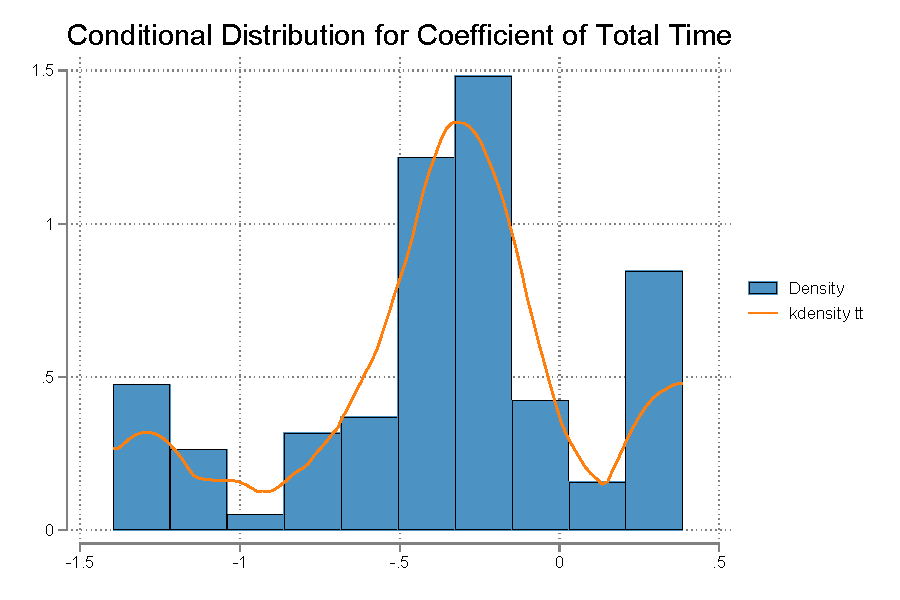
\includegraphics[width=.7\linewidth]{figures/mixRRM_normal_idl}
			\label{fig:mixrrmlnidl}
		\end{figure}\pause
			\item We see some individuals with positive estimates. \pause
		\item To prevent this from happening we can use a bounded distribution...
	\end{itemize}
	

\end{frame}



%%%%%%%%%%%%%%%%%%%%%%%%%%%%%%%%%%%%%%%%%%%%%%%%%%%%%%%%%%%%%
%%%%%%%%%%%%%%%%%%%%%%%%%%%%%%%%%%%%%%%%%%%%%%%%%%%%%%%%%%%%%
%%%%%%%%%%%%%%%%%%%%%%%%%%%%%%%%%%%%%%%%%%%%%%%%%%%%%%%%%%%%%
%%%%%%%%%%%%%%%%%%%%%%%%%%%%%%%%%%%%%%%%%%%%%%%%%%%%%%%%%%%%%

\begin{frame}{Mixed RRM model: Log-normal Distribution}
	
\begin{itemize}
	\item We can use a bounded distribution (negative Log-normal) to force that every individual has a negative parameter for total time.
\end{itemize}
	
	\scalebox{0.77}{\begin{minipage}{\hsize}
			\begin{stlog}
				. gen ntt = -1 * tt
{\smallskip}
. mixrandregret choice  tc , gr(obs) alt(altern) rand(ntt ) ln(1) id(id) ///
> nocons cluster(id)  nrep(100) tech(bhhh) from(b_mixrrm) nolog
{\smallskip}
Case ID variable: obs                          Number of cases    =       1060
Alternative variable: altern                   
Random variable(s): ntt                        
{\smallskip}
                                 (Std. Err. adjusted for  106 clusters in id)
{\smallskip}
Mixed random regret model                       Number of obs     =      3,180
                                                Wald chi2(2)      =    1224.65
Log likelihood = -785.40416                     Prob > chi2       =     0.0000
{\smallskip}
\HLI{13}{\TOPT}\HLI{64}
             {\VBAR}                 OPG
      choice {\VBAR}      Coef.   Std. Err.      z    P>|z|     [95\% Conf. Interval]
\HLI{13}{\PLUS}\HLI{64}
Mean         {\VBAR}
          tc {\VBAR}  -1.217628   .0443379   -27.46   0.000    -1.304529   -1.130727
         ntt {\VBAR}  -1.292678   .1549439    -8.34   0.000    -1.596362   -.9889936
\HLI{13}{\PLUS}\HLI{64}
SD           {\VBAR}
         ntt {\VBAR}   1.362446   .1179392    11.55   0.000      1.13129    1.593603
\HLI{13}{\BOTT}\HLI{64}
{\smallskip}
The sign of the estimated standard deviations is irrelevant: interpret them as
being positive
 \nullskip
			\end{stlog}
	\end{minipage}}
\end{frame}


\begin{frame}{Mixed RRM model: Log-normal Distribution}
	\begin{itemize}
		\item Similarly, we can compute the individual level parameters for the log-normally distributed variable \texttt{tt}.
		\end{itemize}
	
	\scalebox{0.85}{\begin{minipage}{\hsize}
			\begin{stlog}
				. /* Computing Individual Level Parameters */
. qui mixrbeta ntt , nrep(500)  replace saving("${\lbr}graphs_route{\rbr}\\mixRRM_ln_idl") 
{\smallskip}
. use "${\lbr}graphs_route{\rbr}\\mixRRM_ln_idl" , replace
{\smallskip}
. replace ntt = -1 * ntt /*reverse sign for graph*/
(106 real changes made)
{\smallskip}
. list id  ntt  in 1/5 
{\smallskip}
     {\TLC}\HLI{17}{\TRC}
     {\VBAR} id          ntt {\VBAR}
     {\LFTT}\HLI{17}{\RGTT}
  1. {\VBAR}  1   -.04032598 {\VBAR}
  2. {\VBAR}  2   -.08142616 {\VBAR}
  3. {\VBAR}  3   -.04047817 {\VBAR}
  4. {\VBAR}  4   -.04110615 {\VBAR}
  5. {\VBAR}  5   -.04025335 {\VBAR}
     {\BLC}\HLI{17}{\BRC}
 \nullskip
			\end{stlog}
	\end{minipage}}
\end{frame}

\begin{frame}{Mixed RRM model: Log-normal Distribution}
	
\begin{itemize}
\item Individual Level Parameters when total time is assumed to be Log-normally distributed.

	\begin{figure}
		\centering
		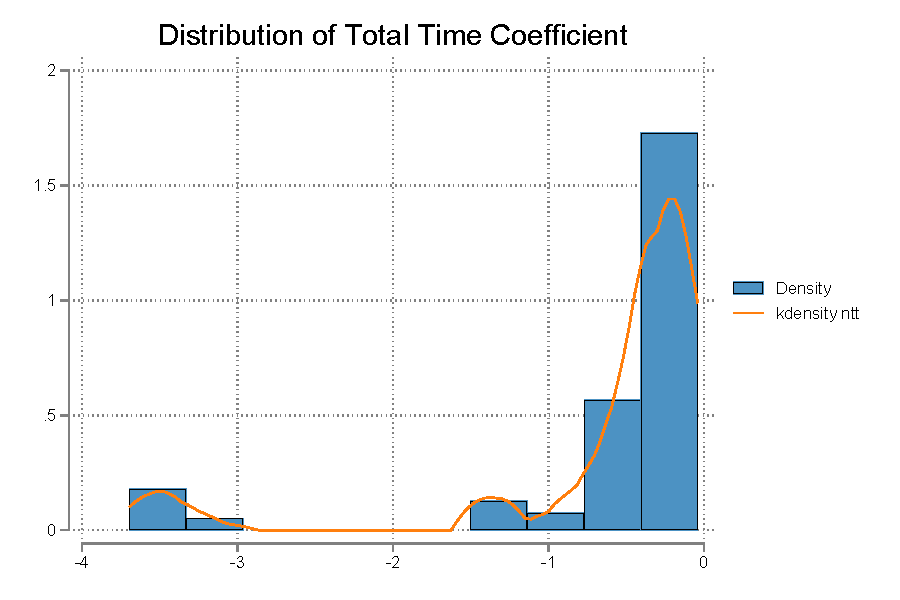
\includegraphics[width=.7\linewidth]{figures/mixRRM_ln_idl}
		\label{fig:mixrrmlnidl}
	\end{figure}
\item Now we observe that the individual level parameters are all negative.

\end{itemize}	

\end{frame}


\begin{frame}{Mixed RRM model: Log-normal Distribution}
	
\begin{itemize}
	\item The parameters we estimated are the mean ($\beta_{tt}$)	and standard deviation ($s_{tt}$) of the natural logarithm of the total time coefficient. 
	\item Hence, the mean, median and variance of log-normal distributed parameter are equal to $\exp(\beta_{tt})$, $\exp(\beta_{tt} + s_{tt}/2)$ and $\exp(\beta_{tt} + s_{tt}/2)\times \sqrt{\exp(s^{2}_{tt})-1}$, respectively.
	\item Finally, we can compute them using \text{nlcom}.
	
\end{itemize}

	
	\scalebox{0.85}{\begin{minipage}{\hsize}
			\begin{stlog}
				. nlcom (mean_time: -1*exp([Mean]_b[ntt ]+0.5*[SD]_b[ntt ]{\caret}2)) ///
> (med_time: -1*exp([Mean]_b[ntt ])) /// 
> (sd_time: exp([Mean]_b[ntt ]+0.5*[SD]_b[ntt ]{\caret}2) * sqrt(exp([SD]_b[ntt ]{\caret}2)-1))
{\smallskip}
   mean_time:  -1*exp([Mean]_b[ntt ]+0.5*[SD]_b[ntt ]{\caret}2)
    med_time:  -1*exp([Mean]_b[ntt ])
     sd_time:  exp([Mean]_b[ntt ]+0.5*[SD]_b[ntt ]{\caret}2) * sqrt(exp([SD]_b[ntt ]{\caret}2)-1)
{\smallskip}
\HLI{13}{\TOPT}\HLI{64}
      choice {\VBAR}      Coef.   Std. Err.      z    P>|z|     [95\% Conf. Interval]
\HLI{13}{\PLUS}\HLI{64}
   mean_time {\VBAR}  -.6747959   .1561273    -4.32   0.000    -.9807998   -.3687919
    med_time {\VBAR}  -.2672598   .0416504    -6.42   0.000     -.348893   -.1856266
     sd_time {\VBAR}   1.564444   .6164874     2.54   0.011     .3561513    2.772737
\HLI{13}{\BOTT}\HLI{64}
 \nullskip
			\end{stlog}
	\end{minipage}}
\end{frame}




\section{Conclusions}

\begin{frame}{Conclusions}
\begin{itemize}
	\item The \texttt{mixrandregret} command extends its predecessor \texttt{randregret} \citep{randregret_2021} by allowing the inclusion of random coefficients in the regret functions.\medskip\pause
	\item The parameters are estimated by Simulated Maximum Likelihood. \medskip\pause
	\item The random parameters can follow either a Normal or Log-normal distribution.\medskip\pause
	\item Additionally, we can compute the individual level parameters using the \texttt{mixrbeta} command. \medskip\pause
	
	\item The programs can be downloaded from \href{https://github.com/ziyue16/mixrandregret}{Ziyue's Github account}. \medskip\pause
	
	\item The example code used in this presentation is available \href{https://github.com/alvarogutyerrez/UKStataConf2022_mixrandregret}{here}.
	
\end{itemize}
\end{frame}







\section{Bibliography}
\begin{frame}{Bibliography}
	%\bibliographystyle{../../randregret_submission/article/sj}
	\bibliography{sj}
\end{frame}




\end{document}